% !TEX TS-program = pdflatex
% !TEX encoding = UTF-8 Unicode

% This is a simple template for a LaTeX document using the "article" class.
% See "book", "report", "letter" for other types of document.

\documentclass[11pt]{article} % use larger type; default would be 10pt

\usepackage[utf8]{inputenc} % set input encoding (not needed with XeLaTeX)
\usepackage{wrapfig}
%%% Examples of Article customizations
% These packages are optional, depending on whether you want the features they provide.
% See the LaTeX Companion or other references for full information.

%%% PAGE DIMENSIONS
\usepackage{geometry} % to change the page dimensions
\geometry{a4paper} % or letterpaper (US) or a5paper or....
% \geometry{margin=2in} % for example, change the margins to 2 inches all round
% \geometry{landscape} % set up the page for landscape
% read geometry.pdf for detailed page layout information

\usepackage{graphicx} % support the \includegraphics command and options
\usepackage{url} % better links representation, o così dicono

% \usepackage[parfill]{parskip} % Activate to begin paragraphs with an empty line rather than an indent

%%% PACKAGES
\usepackage{booktabs} % for much better looking tables
\usepackage{array} % for better arrays (eg matrices) in maths
\usepackage{paralist} % very flexible & customisable lists (eg. enumerate/itemize, etc.)
\usepackage{verbatim} % adds environment for commenting out blocks of text & for better verbatim
\usepackage{subfig} % make it possible to include more than one captioned figure/table in a single float
% These packages are all incorporated in the memoir class to one degree or another...
\usepackage{listings}

\usepackage{graphicx}
\graphicspath{ {./images/} }

%%% HEADERS & FOOTERS
\usepackage{fancyhdr} % This should be set AFTER setting up the page geometry
\pagestyle{fancy} % options: empty , plain , fancy
\renewcommand{\headrulewidth}{0pt} % customise the layout...
\lhead{}\chead{}\rhead{}
\lfoot{}\cfoot{\thepage}\rfoot{}

%%% SECTION TITLE APPEARANCE
\usepackage{sectsty}
\allsectionsfont{\sffamily\mdseries\upshape} % (See the fntguide.pdf for font help)
% (This matches ConTeXt defaults)

\usepackage[usenames,dvipsnames]{xcolor}
\usepackage{hyperref} % To refer a link (website)
\hypersetup{%
  colorlinks=true,% hyperlinks will be coloured
  %linkcolor={BrickRed},% hyperlink text will be green
  linkbordercolor=BrickRed,
  citebordercolor=White,
  urlbordercolor=White,
  runbordercolor=White,
  menubordercolor=White,
  filebordercolor=White,
 % urlcolor={BrickRed},
%filecolor={White},
%citecolor={BrickRed},
allcolors={BrickRed}
%allbordercolors={BrickRed}
}

\makeatletter
\Hy@AtBeginDocument{%
  \def\@pdfborder{0 0 1}% Overrides border definition set with colorlinks=true
  \def\@pdfborderstyle{/S/U/W .5}% Overrides border style set with colorlinks=true
                                % Hyperlink border style will be underline of width 1pt
}
\makeatother

%%% ToC (table of contents) APPEARANCE
\usepackage[nottoc,notlof,notlot]{tocbibind} % Put the bibliography in the ToC
\usepackage[titles,subfigure]{tocloft} % Alter the style of the Table of Contents

\renewcommand{\cftsecfont}{\rmfamily\mdseries\upshape}
\renewcommand{\cftsecpagefont}{\rmfamily\mdseries\upshape} % No bold!

\setlength\parindent{0pt} % Set noindent for the whole document
\newcommand{\ES}{\textcolor{red}}


\usepackage{tikz}
\usetikzlibrary{shapes,trees,fit,decorations.pathreplacing,arrows.meta}

%%% END Article customizations

\begin{document}
%\maketitle

%%% Title page
\begin{titlepage}
	\topskip0pt
	%\vspace*{\fill}
	\centering
	
\includegraphics[width=\textwidth]{logo.png}\\
	\vspace*{1cm}
	\Large \textsc{Second Cycle Degree in Computer Science}
	
	\vspace*{10mm}
	\hrule width \hsize \kern 1mm \hrule width \hsize height 2pt
	\vspace*{5mm}
	\Huge \emph{\textbf{Asset Language}}\\
	\large \emph{\textbf{Compilers and Interpreters  Course Project}}\\
	\large \emph{\textbf{Report on design choices}}
	\vspace*{5mm}
	\hrule width \hsize height 2pt
	\vspace*{1mm}
	\hrule width \hsize \kern 1mm
	
	\vspace*{10mm}
	\begin{minipage}{0.45\textwidth}
		\begin{flushleft} \Large
			\emph{Students:}\\
			\Large \textbf{Giuseppe \textsc{CAPUTO}}\\
			\Large \textbf{Alberto \textsc{PAPARELLA}}
			\Large \textbf{Gabriele \textsc{SPINA}}
		\end{flushleft}
	\end{minipage}	
	\begin{minipage}{0.45\textwidth}
		\begin{flushright} \Large
			\emph{Professor:}\\
			\Large \textbf{Prof. Cosimo \textsc{LANEVE}}
		\end{flushright}
	\end{minipage}
	
	\vspace*{15mm}
	\Large \textsc{Academic Year $2021-2022$}
\end{titlepage}

% Table of contents
\addtocontents{toc}{~\hfill\textbf{Page}\par}	% https://texblog.org/2011/09/09/10-ways-to-customize-tocloflot/
\clearpage
\tableofcontents
\thispagestyle{empty}
\addtocontents{toc}{\protect\thispagestyle{empty}}	% http://tex.stackexchange.com/questions/2995/removing-page-number-from-toc
\newpage

\section{Introduction}
This report will discuss the implementation choices related to the design of a compiler and relative interpreter for a specific programming language, called \emph{AssetLan} (i.e., Asset Language). 

\medskip

\emph{Asset Language} is a simple imperative language with assets, where parameters could be either {\emph standard} or {\emph assets}, with recursion and without mutual recursion. Regarding the semantics, two types of operations are allowed on a parameter defined as an {\emph asset}, and it is legit to use them only in a function. To this aim, a function can be declared  with {\emph assets} in the following way:
\begin{verbatim}
    void f(int a, bool b)[asset u, asset v] { body }
\end{verbatim} 
and called as: 
\begin{verbatim}
    f(5,true)[x,y]
\end{verbatim}
At the time of the call, assets \verb|x| and \verb|y| are emptied and their values are assigned respectively to the formal parameters \verb|u| and \verb|v|; therefore, after the call, the values of assets \verb|x| and \verb|y| are both equal to 0.

\medskip

The value of an \emph{asset} can \textbf{only} be moved using the two aforementioned operations, more specifically: 
\begin{itemize}
\item \textbf{Move operation} (\verb|x -o z|): the value of the parameter \verb|x| is added to the value of the parameter \verb|z| and stored in \verb|z|, then the value of the parameter \verb|x| is set to 0;
\item \textbf{Transfer operation} (\verb|transfer x|): this operation transfers the value of the asset \verb|x| to the caller of the function, then its value is set to 0.
\end{itemize}

\section{Usage}

\subsection{Launching from command line}

Tu use the compiler, go to folder \verb|/src| and compile all java files in the sub directories with \verb|javac */*.java| (it is assumed that antlr4 has already been added to java classpath).
To execute the compiler on a file with \verb|.al| extension, place the file in the \verb|/src| directory and call the Test class, which contains the main function, as follows: \verb|java mainpackage.Test input.al|, where \verb|input.al| is an example of file name.

\subsection{Launching from IDE}
To launch the analysis from an IDE (e.g., Eclipse), open the \verb|src| folder as a new project and add antlr4 to the build path according to the IDE settings. Then, create a new launch configuration to tell the IDE where the main class is, which can be found int \verb|/src/mainpackage/Test.java|, and the command line arguments, in this case the input file with \verb|.al| extension (e.g., \verb|input.al|).

\section{Exercises}
\label{sec:exercices}
The following exercises were used as guidelines/objectives for the design of the compiler:

\begin{enumerate}
\item \textbf{Lexical Errors}: the lexical analyzer must return the list of lexical errors in an output file. 
\item \textbf{Symbol Table}: implement the table of symbols as a list of hash-tables or a hash-table of lists, in order to check errors related to:
\begin{itemize}
\item undeclared functions/variables;
\item multiple declarations of functions/variables in the same environment.
\end{itemize}
\end{enumerate}

\subsection{Lexical Errors}
In order to redirect the errors of the lexer to an output (log) file, one should override the base error handling strategy of ANTLR, which, by default, redirects the errors to the standard error (i.e., the console). To change the destination and, eventually, the content of error messages, one should provide an implementation of an \textsc{ANTLRErrorListener} subclass; Figure~\ref{fig:err} shows the structure of the classes involved in the error handling phase.
\begin{figure}
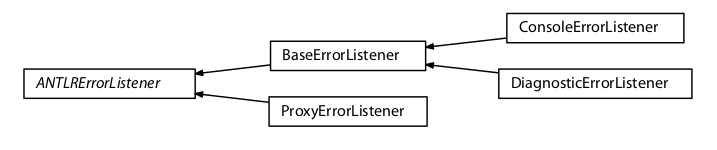
\includegraphics[width=0.95\textwidth]{errorListener.png}
\caption{Internal structure for error handling\cite{reference}.}
\label{fig:err}
\end{figure}   
More specifically, \textsc{ANTLRErrorListener} provides a \textsc{syntaxError()} method that applies to both the lexer and the parser, which receives all sorts of information about the location of the error, as well as the error message and which recognizer caught the error (i.e., if the error occurred during the lexical or the syntactic analysis).   

\medskip

The proposed solution consists of a class, called \textsc{TestLexerListner}, which extends the \textsc{BaseErrorListener} class in order to override the \textsc{syntaxError()} method and redirect his output to a log file, named \verb|log.txt|. Furthermore, for each error, it prints the date and time at which it occurred, so that it is possible to distinguish between errors coming from different compilation executions. 

\medskip

At this point, one can simply remove the \textsc{ConsoleErrorListener} (i.e., the default strategy) for the lexer and bind the custom listener instead, adding the following lines to the main function intended to launch the analysis and relative compilation (in the project, defined in the \verb|Test| class, implemented in \verb|src/mainpackage/Test.java|):
\begin{lstlisting}
    lexer.removeErrorListeners();
    lexer.addErrorListener(new TestLexerListener());
\end{lstlisting}

\medskip

A lexical error is defined as a sequence of characters that does not match the pattern of any token. In our language, this can only happen when the lexer founds a character which is not defined in the grammar, and therefore it cannot derive the relative token. 

\medskip

The following examples show the output messages printed to the \verb|log.txt| file when a lexical error is found:
\begin{enumerate}
\item
	\begin{itemize}
		\item Code tested: \begin{lstlisting}
int a = "s";   
f()[]
		\end{lstlisting}
		\item Output on \textsc{log.txt}: \begin{lstlisting}
20-04-2022 15:33:13: 
    Found Lexical error at line 1 at position 8: 
    token recognition error at: '"'
20-04-2022 15:33:14: 
    Found Lexical error at line 1 at position 10: 
    token recognition error at: '"'
		\end{lstlisting}
	\end{itemize}
\item
\begin{itemize}
\item Code tested: \begin{lstlisting}
int main()[]{}
ma$n()[]
\end{lstlisting}
\item Output on \textsc{log.txt}: \begin{lstlisting}
20-04-2022 15:48:56: 
    Found Lexical error at line 2 at position 2: 
    token recognition error at: '$'
\end{lstlisting}
\end{itemize}
\item
	\begin{itemize}
	\item Code tested: \begin{lstlisting}
int a:
f()[]
	\end{lstlisting}
	\item Output on \textsc{log.txt}: \begin{lstlisting}
20-04-2022 15:55:52: 
    Found Lexical error at line 1 at position 5: 
    token recognition error at: ':'
	\end{lstlisting}
	\end{itemize}
\end{enumerate}

\clearpage

\subsection{Symbol Table}
The choice of the data structure for the symbol table fell on the list of hash-tables because an excessive level of nesting in the code is not expected. This is due to the fact that the grammar of the language does not allow the definition of {code blocks}~\cite{codeblocks} (i.e., using curly brackets to define a new scope explicitly, as in SimpLanPlus) and mutual recursion is not conceived; therefore, the only way to enter in a new scope is the definition of a new function. That leads to a language that frequently enters and exits scopes, so it has been decided to opt for a solution that could reduce the complexity of these particular operations, accepting a higher complexity for the look-up of an identifier. Given the implementation of a symbol table as a list of hash-tables, the cost for entering and exiting a scope is \(O(1)\), while the cost for the look-up operation is \(O(depth_{nesting})\).

\medskip

The symbol table has been declared as a private field in a specific class, called \textsc{Environment}. In order to access/modify it, the following methods have been implemented:
\begin{itemize}
\item \textsc{enterScope()}: increases the nesting level and adds a new entry (i.e., an hash-table) to the list. 
\item \textsc{exitScope()}: decreases the nesting level and removes the last hash-table from the list.
\item \textsc{getScope(nestingLevel)}/\textsc{getCurrentScope()}: returns the scope relative to the specified nesting level/relative to the current nesting level.
\item \textsc{addEntry(type, identifier)}: adds an entry with specified type and id to the hash-table relative to the current scope.
\item \textsc{getNestingLevel()}: getter for nesting level field.
\item \textsc{checkDeclaration(identifier, nestingLevel)}: checks if the symbol has been declared in the specified scope (retrieved from nesting level). 
\item \textsc{lookup(identifier)}: look-up for the declaration of a given id in the current scope or an enclosing one. 
\end{itemize}

\medskip

To manage the symbol table, it is necessary to visit the Abstract Syntax Tree in order to insert the declarations of variables / functions / assets within the data structure. To this aim, the \textsc{AssetLanBaseVisitor} class has been extended to override the auto-generated methods meant to visit the AST. For each rule in the grammar, it has been defined a new class representing the relative node of the tree with its specific components and methods. Among these, \textsc{checkSemantics(environment)} searches for semantic errors, such as multiple declarations of variables and functions, as well as undeclared ones.

\medskip

In the \textsc{AssetLanBaseVisitor} there is a visit method for each rule in the grammar meant to construct the relative node with the help of the ANTLR's rule contexts. 

\medskip

The following example shows the output for a program which contains both types of errors (one multiple declaration error and one usage of undeclared variable error):

\begin{enumerate}
\item
	\begin{itemize}
		\item Code tested: \begin{lstlisting}
int a;
asset b;
int main(int a)[asset c]{
    int a;
    c -o d;
}
main()[2]
		\end{lstlisting}
		\item Output on console: \begin{lstlisting}
You had: 2 errors:
	Error when declaring variable of id a,
	Id already used for declaration in the same scope
	
	Asset d has not been declared
		\end{lstlisting}
		
	The first error is caused by the declaration of variable \verb|a| at line 4, which has already been declared as parameter in the function.
	The second error is caused by the fact that asset \verb|d| has never been declared.
	\end{itemize}
\end{enumerate}

\section{Conclusion}
In this report, the implementation choices for the development of a compiler for the Asset Language have been discussed.

\medskip

Regarding the lexical error handling strategy, a common lexical error regards the length of integer number definitions. It has been decided to keep the default error handling strategy provided by Java instead of changing the grammar limiting the length of numbers.

\medskip

There are several ways to improve the given solutions. Among these, one could add information about the line where an identifier has been declared to the symbol table, in order to improve the error message. In this version, the symbol table is implemented in a way that does not handle type checking, so the look-up operation for an identifier does not take into account the type of the variable / function or the kind of operation in which it is involved.

\medskip

Also, the bytecode generation and relative interpreter are missing.

\clearpage

\begin{thebibliography}{9}
\bibitem{reference}
Parr, Terence (2013) , The definitive ANTLR 4 reference.

\bibitem{basics}
Mogensen, {Torben {\AE}gidius} (1999), Basics of Compiler Design, Kursusbog 

\bibitem{patterns}
Parr, Terence (2013) , Language Implementation Patterns: Create Your Own Domain-Specific and General Programming Languages.

\bibitem{codeblocks}
Wikipedia contributors. Block (programming). Wikipedia, The Free Encyclopedia. January 12, 2022, 03:55 UTC. 
\end{thebibliography}

\end{document}
